\documentclass{standalone}
\usepackage{graphicx}	
\usepackage{amssymb, amsmath}
\usepackage{color}

\usepackage{tikz}
\usetikzlibrary{intersections, backgrounds, patterns, patterns.meta}
\usepackage{pgfmath}

\definecolor{light}{RGB}{220, 188, 188}
\definecolor{mid}{RGB}{185, 124, 124}
\definecolor{dark}{RGB}{143, 39, 39}
\definecolor{highlight}{RGB}{180, 31, 180}
\definecolor{gray10}{gray}{0.1}
\definecolor{gray20}{gray}{0.2}
\definecolor{gray30}{gray}{0.3}
\definecolor{gray40}{gray}{0.4}
\definecolor{gray60}{gray}{0.6}
\definecolor{gray70}{gray}{0.7}
\definecolor{gray80}{gray}{0.8}
\definecolor{gray90}{gray}{0.9}
\definecolor{gray95}{gray}{0.95}

\newcommand*{\offset}{0.025}

\begin{document}

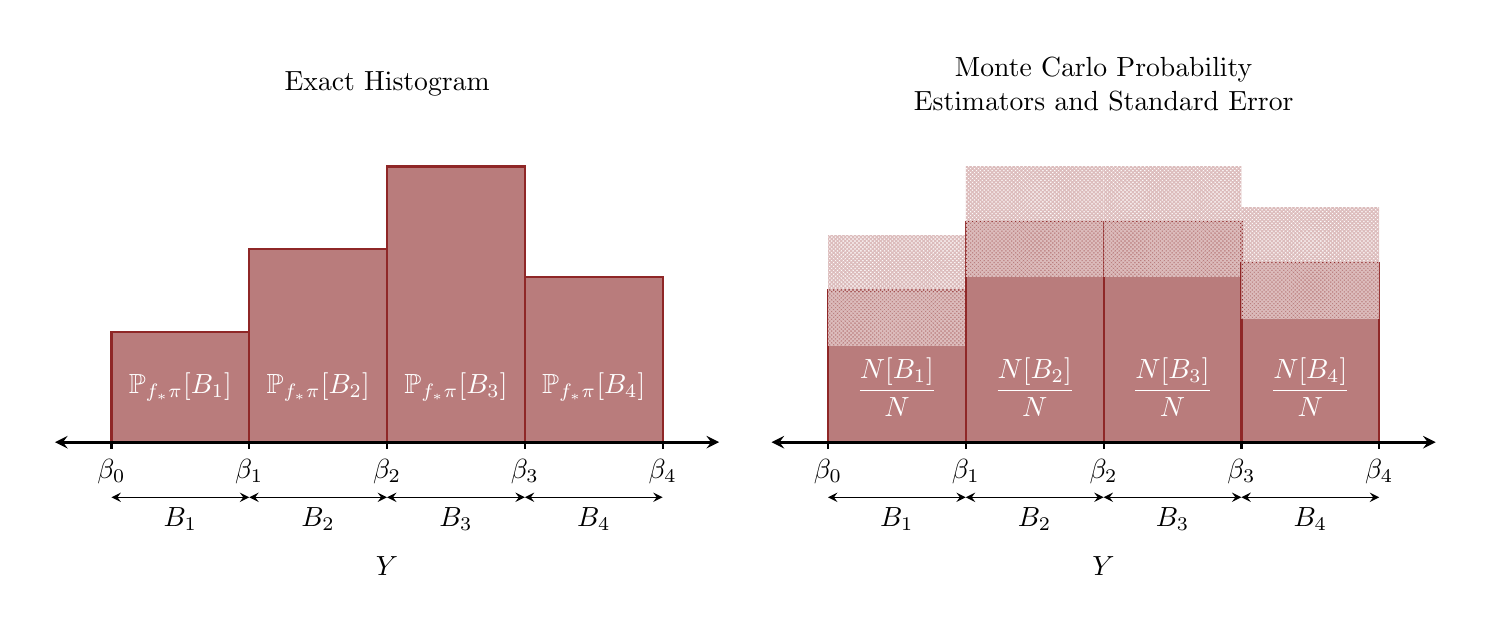
\begin{tikzpicture}[scale=0.35, thick]

\begin{scope}[shift={(0, 0)}]
  \draw[white] (-13, -6) rectangle (13, 15);
  
  \node at (0, 13) { Exact Histogram };

  \draw [<->, >=stealth, line width=0.5] (-10, -2) -- (-5, -2)
  node[below, midway]  { $B_{1}$ }; 
  
  \filldraw [fill=mid, draw=dark] (-10, 0) rectangle (-5, 4);
  \node[text=white] at (-7.5, 2) { $\mathbb{P}_{f_{*} \pi}[B_{1}]$ };
  
  \draw [<->, >=stealth, line width=0.5] (-5, -2) -- (0, -2)
  node[below, midway]  { $B_{2}$ }; 
  
  \filldraw [fill=mid, draw=dark] (-5, 0) rectangle (0, 7);
  \node[text=white] at (-2.5, 2) { $\mathbb{P}_{f_{*} \pi}[B_{2}]$ };

  \draw [<->, >=stealth, line width=0.5] (0, -2) -- (5, -2)
  node[below, midway]  { $B_{3}$ };
  
  \filldraw [fill=mid, draw=dark] (0, 0) rectangle (5, 10);
  \node[text=white] at (2.5, 2) { $\mathbb{P}_{f_{*} \pi}[B_{3}]$ };
  
  \draw [<->, >=stealth, line width=0.5] (5, -2) -- (10, -2)
  node[below, midway]  { $B_{4}$ };
  
  \filldraw [fill=mid, draw=dark] (5, 0) rectangle (10, 6);
  \node[text=white] at (7.5, 2) { $\mathbb{P}_{f_{*} \pi}[B_{4}]$ };
  
  \draw [<->, >=stealth, line width=1] (-12.05, 0) -- +(24.1, 0);
  \node[] at (0, -4.5) { $Y$ };
  
  \draw [] (-10, 0) -- +(0, -0.25)
  node [below] { $\beta_{0}$ };
  
  \draw [] (-5, 0) -- +(0, -0.25)
  node [below] { $\beta_{1}$ };
  
  \draw [] (0, 0) -- +(0, -0.25)
  node [below] { $\beta_{2}$ };
  
  \draw [] (5, 0) -- +(0, -0.25)
  node [below] { $\beta_{3}$ };
  
  \draw [] (10, 0) -- +(0, -0.25)
  node [below] { $\beta_{4}$ };
  
\end{scope}


\begin{scope}[shift={(26, 0)}]
  \draw[white] (-13, -6) rectangle (13, 15);
  
  \node[align=center] at (0, 13) { Monte Carlo Probability\\Estimators and Standard Error };

  % Bin 1
  \draw [<->, >=stealth, line width=0.5] (-10, -2) -- (-5, -2)
  node[below, midway]  { $B_{1}$ }; 
  
  \filldraw [fill=mid, draw=dark] (-10, 0) rectangle (-5, 4 + 1.5);
  \node[text=white] at (-7.5, 2) { $\displaystyle \frac{N[B_{1}]}{N}$ };
  
  \fill[pattern={Hatch[angle=45,distance=1, line width=0.5]}, pattern color=light] 
    (-10, 5.5 - 2) rectangle (-5, 5.5 + 2);
  
  % Bin 2
  \draw [<->, >=stealth, line width=0.5] (-5, -2) -- (0, -2)
  node[below, midway]  { $B_{2}$ }; 
  
  \filldraw [fill=mid, draw=dark] (-5, 0) rectangle (0, 7 + 1);
  \node[text=white] at (-2.5, 2) { $\displaystyle \frac{N[B_{2}]}{N}$ };

  \fill[pattern={Hatch[angle=45,distance=1, line width=0.5]}, pattern color=light] 
    (-5, 8 - 2) rectangle (0, 8 + 2);
     
  % Bin 3
  \draw [<->, >=stealth, line width=0.5] (0, -2) -- (5, -2)
  node[below, midway]  { $B_{3}$ };
  
  \filldraw [fill=mid, draw=dark] (0, 0) rectangle (5, 10 - 2);
  \node[text=white] at (2.5, 2) { $\displaystyle \frac{N[B_{3}]}{N}$ };
  
  \fill[pattern={Hatch[angle=45,distance=1, line width=0.5]}, pattern color=light] 
     (0, 8 - 2) rectangle (5, 8 + 2);
  
  % Bin 4
  \draw [<->, >=stealth, line width=0.5] (5, -2) -- (10, -2)
  node[below, midway]  { $B_{4}$ };
  
  \filldraw [fill=mid, draw=dark] (5, 0) rectangle (10, 6 + 0.5);
  \node[text=white] at (7.5, 2) { $\displaystyle \frac{N[B_{4}]}{N}$ };
  
  \fill[pattern={Hatch[angle=45,distance=1, line width=0.5]}, pattern color=light] 
     (5, 6.5 - 2) rectangle (10, 6.5 + 2);
     
  % Axis
  \draw [<->, >=stealth, line width=1] (-12.05, 0) -- +(24.1, 0);
  \node[] at (0, -4.5) { $Y$ };
  
  \draw [] (-10, 0) -- +(0, -0.25)
  node [below] { $\beta_{0}$ };
  
  \draw [] (-5, 0) -- +(0, -0.25)
  node [below] { $\beta_{1}$ };
  
  \draw [] (0, 0) -- +(0, -0.25)
  node [below] { $\beta_{2}$ };
  
  \draw [] (5, 0) -- +(0, -0.25)
  node [below] { $\beta_{3}$ };
  
  \draw [] (10, 0) -- +(0, -0.25)
  node [below] { $\beta_{4}$ };
  
\end{scope}

  
\end{tikzpicture}

\end{document}  